\documentclass[11pt,a4paper]{article}
\usepackage[utf8]{inputenc}
\usepackage[T1]{fontenc}
% \usepackage[document]{ragged2e}
% \usepackage[a4paper, total={5in, 8in}]{geometry}
\usepackage[english]{babel}
\usepackage{amsmath, amsthm, amssymb, amsfonts}
\usepackage{enumerate}
\usepackage{graphicx}
\usepackage{fancyhdr}
\usepackage{booktabs}
\usepackage{csvsimple}
\usepackage{longtable}
\usepackage{textcomp}
\usepackage{float}
\usepackage[colorlinks=true,breaklinks=false]{hyperref}
\usepackage{listings}
\usepackage[norelsize,ruled,vlined]{algorithm2e}
\usepackage{csquotes}
\usepackage{url}
\usepackage{ifthen}
\usepackage{keyval}
\usepackage{etoolbox}
\usepackage{etex}
\usepackage{datetime}
\usepackage{eurosym}
\usepackage{tikz}
\usepackage{wrapfig}
\usepackage{paralist}
\usepackage[backend=bibtex]{biblatex}
\usepackage{xcolor}
\usepackage{caption}
\DeclareCaptionFont{white}{\color{white}}
\DeclareCaptionFormat{listing}{\colorbox[cmyk]{0.43, 0.35, 0.35,0.01}{\parbox{\textwidth}{\hspace{15pt}#1#2#3} } }
\captionsetup[lstlisting]{format=listing, labelfont=white, textfont=white, singlelinecheck=false, margin=0pt, font={bf,footnotesize} }

\hyphenpenalty=10000
% \pretolerance=9999
% \tolerance=9999
% \emergencystretch=0pt
\addbibresource{project.bib}
% \setlength{\parindent}{2em}
\renewcommand{\baselinestretch}{1.1}
\newcommand{\scalafmt}{\texttt{scalafmt}}

% Single spacing after dots and colons
\frenchspacing
\hyphenation{scalafmt}
\hyphenation{ClangFormat}
% \hyphenation{DSLVirtualization}
% \hyphenation{ReificationTransformation}

%%%%%%%%%%%%%%%%%%%%%%%%%%%%%%%%%%%%%%%%%%%%%%%%%%%%%%%%%%%%%
%                        Setup
%%%%%%%%%%%%%%%%%%%%%%%%%%%%%%%%%%%%%%%%%%%%%%%%%%%%%%%%%%%%%

\begin{document}
\raggedright

\definecolor{dkgreen}{rgb}{0,0.6,0}
\definecolor{gray}{rgb}{0.5,0.5,0.5}
\definecolor{mauve}{rgb}{0.58,0,0.82}

\lstdefinestyle{scala}{
  language=Scala,
  aboveskip=3mm,
  basicstyle=\scriptsize\ttfamily,
  belowskip=3mm,
  breakatwhitespace=false,
  showspaces=false,
  showlines=true,
  columns=flexible,
  keepspaces=true,
  commentstyle=\color{dkgreen},
  keywordstyle=\color{blue},
  numbers=left,
  numberstyle=\tiny\color{gray},
  showstringspaces=false,
  stepnumber=1,
}


\definecolor{dkgreen}{rgb}{0,0.6,0}
\definecolor{gray}{rgb}{0.5,0.5,0.5}
\definecolor{mauve}{rgb}{0.58,0,0.82}

\lstset{language=Scala,
  aboveskip=3mm,
  basicstyle={\small\ttfamily},
  belowskip=3mm,
  breakatwhitespace=true,
  breaklines=true,
  columns=flexible,
  commentstyle=\color{dkgreen},
  keywordstyle=\color{blue},
  numbers=left,
  numberstyle=\tiny\color{gray},
  showstringspaces=false,
  stepnumber=1,
  stringstyle=\color{mauve},
  tabsize=2,
}

\usetikzlibrary{calc,trees,positioning,arrows,chains,shapes.geometric,%
    decorations.pathreplacing,decorations.pathmorphing,shapes,%
    matrix,shapes.symbols}
\tikzset{>=stealth',
  punktchain/.style={rectangle,
    rounded corners,
    % fill=black!10,
    draw=black, very thick,
    text width=12.5em,
    minimum height=2.5em,
    text centered,
    on chain},
  every join/.style={->, shorten >=2pt},
}


% Example of title page for the projects carried out within the lasec

% Simply include it in your mastex tex file:
%        % Example of title page for the projects carried out within the lasec

% Simply include it in your mastex tex file:
%        % Example of title page for the projects carried out within the lasec

% Simply include it in your mastex tex file:
%        \input{cover}


% Updated March 2006 (SP)


\newcommand{\logoepfl}[0]{
  \begin{center}
    
\includegraphics[width=4cm]{logo_epfl_coul.eps}
  \end{center}
  \vspace{0.3cm}
  \hrule
}
\newcommand{\logolasec}[0]{
  \vspace{1cm}
  \hrule
  \begin{center}
    \includegraphics[width=4.5cm]{logo_lasec_coul.eps}
  \end{center}
}
\newcommand{\project}[1]{
  \begin{center}
    \large{#1}
  \end{center}
  \vspace{1cm}
}
\newcommand{\department}[1]{
  \begin{center}
    \large{#1}
  \end{center}
}
\newcommand{\supervisor}[3]{
  \begin{center}
    \begin{normalsize}{
        \bf #1}\\#2\\#3
    \end{normalsize}
  \end{center}
}
\renewcommand{\author}[1]{
  \begin{center}
    \Large{#1}
  \end{center}
  \vspace{0.5cm}
}
\renewcommand{\title}[1]{
  \vspace{3cm}
  \begin{center}
    \huge{#1}
  \end{center}
  \vspace{1.7cm}
}
\renewcommand{\date}[2]{
  \begin{center}
    \normalsize{#1 #2}
  \end{center}
  \vspace{0.5cm}
}


\thispagestyle{empty}


% begin title page
  \logoepfl

  \title{scalafmt: yet another approach \\ to code formatting}

  \author{Ólafur Páll Geirsson}
  \department{School of Computer and Communication Sciences}
  \project{Master's Thesis}

  \date{June}{2015}

  \begin{center}
    \begin{tabular}{cc}
      \begin{tabular}{p{4.0cm}}
        \supervisor{Responsible}{Prof. Martin Odersky}{EPFL / LAMP}
      \end{tabular}&
      \begin{tabular}{p{4.0cm}}
        \supervisor{Supervisor}{Eugene Burmako}{EPFL / LAMP}
      \end{tabular}
    \end{tabular}
  \end{center}

% end title page




% Updated March 2006 (SP)


\newcommand{\logoepfl}[0]{
  \begin{center}
    
\includegraphics[width=4cm]{logo_epfl_coul.eps}
  \end{center}
  \vspace{0.3cm}
  \hrule
}
\newcommand{\logolasec}[0]{
  \vspace{1cm}
  \hrule
  \begin{center}
    \includegraphics[width=4.5cm]{logo_lasec_coul.eps}
  \end{center}
}
\newcommand{\project}[1]{
  \begin{center}
    \large{#1}
  \end{center}
  \vspace{1cm}
}
\newcommand{\department}[1]{
  \begin{center}
    \large{#1}
  \end{center}
}
\newcommand{\supervisor}[3]{
  \begin{center}
    \begin{normalsize}{
        \bf #1}\\#2\\#3
    \end{normalsize}
  \end{center}
}
\renewcommand{\author}[1]{
  \begin{center}
    \Large{#1}
  \end{center}
  \vspace{0.5cm}
}
\renewcommand{\title}[1]{
  \vspace{3cm}
  \begin{center}
    \huge{#1}
  \end{center}
  \vspace{1.7cm}
}
\renewcommand{\date}[2]{
  \begin{center}
    \normalsize{#1 #2}
  \end{center}
  \vspace{0.5cm}
}


\thispagestyle{empty}


% begin title page
  \logoepfl

  \title{scalafmt: yet another approach \\ to code formatting}

  \author{Ólafur Páll Geirsson}
  \department{School of Computer and Communication Sciences}
  \project{Master's Thesis}

  \date{June}{2015}

  \begin{center}
    \begin{tabular}{cc}
      \begin{tabular}{p{4.0cm}}
        \supervisor{Responsible}{Prof. Martin Odersky}{EPFL / LAMP}
      \end{tabular}&
      \begin{tabular}{p{4.0cm}}
        \supervisor{Supervisor}{Eugene Burmako}{EPFL / LAMP}
      \end{tabular}
    \end{tabular}
  \end{center}

% end title page




% Updated March 2006 (SP)


\newcommand{\logoepfl}[0]{
  \begin{center}
    
\includegraphics[width=4cm]{logo_epfl_coul.eps}
  \end{center}
  \vspace{0.3cm}
  \hrule
}
\newcommand{\logolasec}[0]{
  \vspace{1cm}
  \hrule
  \begin{center}
    \includegraphics[width=4.5cm]{logo_lasec_coul.eps}
  \end{center}
}
\newcommand{\project}[1]{
  \begin{center}
    \large{#1}
  \end{center}
  \vspace{1cm}
}
\newcommand{\department}[1]{
  \begin{center}
    \large{#1}
  \end{center}
}
\newcommand{\supervisor}[3]{
  \begin{center}
    \begin{normalsize}{
        \bf #1}\\#2\\#3
    \end{normalsize}
  \end{center}
}
\renewcommand{\author}[1]{
  \begin{center}
    \Large{#1}
  \end{center}
  \vspace{0.5cm}
}
\renewcommand{\title}[1]{
  \vspace{3cm}
  \begin{center}
    \huge{#1}
  \end{center}
  \vspace{1.7cm}
}
\renewcommand{\date}[2]{
  \begin{center}
    \normalsize{#1 #2}
  \end{center}
  \vspace{0.5cm}
}


\thispagestyle{empty}


% begin title page
  \logoepfl

  \title{scalafmt: yet another approach \\ to code formatting}

  \author{Ólafur Páll Geirsson}
  \department{School of Computer and Communication Sciences}
  \project{Master's Thesis}

  \date{June}{2015}

  \begin{center}
    \begin{tabular}{cc}
      \begin{tabular}{p{4.0cm}}
        \supervisor{Responsible}{Prof. Martin Odersky}{EPFL / LAMP}
      \end{tabular}&
      \begin{tabular}{p{4.0cm}}
        \supervisor{Supervisor}{Eugene Burmako}{EPFL / LAMP}
      \end{tabular}
    \end{tabular}
  \end{center}

% end title page



\begin{abstract}
  Code formatters bring many benefits to software development such as enforcing a consistent coding style across teams, more effective code reviews and enabling automated large-scale refactoring.
  % Still, code formatters can be tricky to get right.
  This thesis addresses how to develop a code formatter for the Scala programming language.
  We present scalafmt, an opinionated Scala code formatter that captures many popular Scala idioms and coding styles.
  This thesis introduces language-agnostic algorithms and tooling that scalafmt uses to implement advanced features such as line wrapping and configurable vertical alignment.
  We have validated that these techniques work well in practice.
  Scalafmt has been installed over 6.500 times in only 3 months and
  several popular open-source libraries have chosen to reformat their codebases with scalafmt.
\end{abstract}
% \newpage
\vspace{1in}
\renewcommand{\abstractname}{Útdráttur}

\begin{abstract}
  Kóðasniðlar (e. code formatters) eru nytsamleg tól í hugbúnaðarþróun.
  Helstu kostir kóðasniðla eru meðal annars að geta sjálfvirkt framfylgt samræmdum kóðastíl, skilvirkari kóðaumsögnum og gera kleift að endurskipleggja stór forritasöfn.
  Þetta verkefni fjallar um að þróa kóðasniðil fyrir Scala forritunarmálið.
  Við kynnum scalafmt, kóðasniðil fyrir Scala sem fangar marga vinsæla Scala kóðastíla og forritunartiltæki.
  Þetta verkefni kynnir reiknirit og gagnagrindur til að útfæra háþróaða eiginlega eins og að brjóta langar forritunarskipanir á einni línu niður í margar línur og raða tóka af svipuðu tagi frá mörgum línum þannig að tókarnir liggi á sama lóðrétta dálki.
  Aðferðir sem kynntar eru í þessu verkefni hafa sannað sig í verki.
  Scalafmt hefur verið halað niður yfir 6.500 sinnum á eingöngu 3 mánuðum og fjöldi af vinsælum opnum forritasöfnum hafa kosið að sníða kóðann sinn með scalafmt.
\end{abstract}

\begin{abstract}
  Code formatters bring many benefits to software development, yet they can be tricky to get right.
  This thesis addresses the problem of developing a code formatter for the Scala programming language.
  We present scalafmt, an opinionated Scala code formatter that captures many popular Scala idioms and coding styles.
  Scalafmt has been installed over 6.000 times since its initial release 3 months ago, adopted by several open-source libraries and attracted a vibrant community of external contributors.
  Our work has been limited to formatting Scala code.
  Still, this thesis presents algorithms and tooling that we believe can be of interest to the development of code formatters for other programming languages.
\end{abstract}
\tableofcontents
\lstlistoflistings
\listofalgorithms
\listoffigures
\listoftables

\setlength{\parskip}{1em}
\section{Introduction} % (fold)
\label{sec:Introduction}
\lstset{style=scala}
Without code formatters, software developers are responsible for manipulating all syntactic trivia in their programs.
What is syntactic trivia?
Consider the Scala code snippets in listings~\ref{lst:unformatted} and~\ref{lst:formatted1}.

\begin{minipage}{.45\textwidth}
\lstinputlisting[label={lst:unformatted}, caption=Unformatted code]{code/unformatted.scala}
\end{minipage}
\hfil
\begin{minipage}{.45\textwidth}
\lstinputlisting[label={lst:formatted1}, caption=Formatted code]{target/formatted1.scala}
\end{minipage}

Both snippets represent the same application.
The only difference lies in where the programmer has chosen to break lines.
Characters such as spaces and line breaks that do not affect the execution of the program are syntactic trivia.
Although syntactic trivia has no meaning for the execution of the program, listing~\ref{lst:formatted1} is arguably easier to understand, maintain and extend for the software developer.
A code formatter is a tool that automatically converts a program such as in listing~\ref{lst:unformatted} into a readable and maintainable program such as in listing~\ref{lst:formatted1}.
Code formatting brings several benefits to software development.

Code formatting enables automated large-scale refactoring.
Google used ClangFormat\autocite{jasper_clangformat_2013}, a C++ code formatter,
in the process of migrating a large legacy C++98 codebase to use the modern C++11 standard\autocite{wright_large-scale_2013}.
The automatically refactored code was formatted with ClangFormat to ensure that it adhered to Google's strict coding style\autocite{_google_????}.
Similar migrations can be expected in the near future for the Scala community once new dialects, such as Dotty\autocite{rompf_f_2015}, gain popularity.

Code formatting is valuable in collaborative coding environments.
The Scala.js project\autocite{_scala.js_????} has over 40 contributors and the Scala.js coding style\autocite{doeraene_scala.js_2015} --- which each Scala.js contributor is expected to know by heart --- is defined at a whopping 2.600 word count.
Each contributed patch is manually verified against the coding style by the project maintainers.
This adds a burden on both contributors and maintainers.
Several prominent Scala community members have raised this issue.
ENSIME\autocite{_ensime_????} is a popular Scala interaction mode for text editors such as Vim and Emacs.
Sam Halliday, an ENSIME maintainer, says ``I don't have time to talk about formatting in code reviews. I want the machine to do it so I can focus on the design.''\autocite{halliday_i_2016-1}.
Akka\autocite{_akka_????} is a popular concurrent and distributed programming library for Scala with over 300 contributors.
Viktor Klang, a maintainer of Akka, suggests a better alternative ``Code style should not be enforced by review, but by automate rewriting. Evolve the style using PRs against the rewriting config.''.\autocite{klang_code_2016}.

With scalafmt, we hope to relieve Scala developers from the burden of manipulating syntactic trivia so they can instead direct their full attention to writing correct, maintainable and fast code.

\subsection{Research objective}
% Code formatters bring several benefits to software development.
% However, the Scala community has enjoyed limited benefits from the 
% Can we develop a code formatter for the Scala programming language

What algorithms and data structures allow us to develop a code formatter for the Scala programming language with the following properties?
\begin{itemize}
  \item \textbf{Maximum line length setting}: a code formatter with a maximum line length setting ensures that each line in the formatted output contains no more than a certain number of characters.
    Many coding styles enforce a maximum line length in order to make code readable from different environments such as small split screens and code review interfaces.
  \item \textbf{Opinionated}:
    An opinionated setting is a prerequisite to enforce a uniform coding style.
    An opinionated code formatter takes liberty to disregard line breaks and other formatting decisions in the original source input to ensure that formatted source files follow the same line breaking conventions.
  \item \textbf{Vertical alignment}: vertical alignment is a formatting convention where redundant whitespace is added before a token to align it on the same vertical column as similar tokens from other lines. Many Scala coding styles enforce vertical alignment to enhance code readability.
  \item \textbf{Performance}: Users expect code formatters to run fast.
    In the most demanding settings, a code formatter needs to be able to format thousands of lines of code in at most a few hundred milliseconds.

\end{itemize}

\subsection{Contributions}
The main contributions presented in this thesis are the following:
\begin{itemize}
  \item language-agnostic algorithms and data structures to implement line
    wrapping with a maximum line length setting --- in our opinion, the most
    challenging part of developing a code formatter --- as well as configurable
    vertical alignment.
    This work is presented in section~\ref{sec:algorithms}.
  \item methods to optimize and test the developed algorithms.
    This work is presented in section~\ref{sec:tooling}.
  \item practical validation of developed algorithms and methods with the scalafmt code formatter.
    The empirical results of this validation are presented in section~\ref{sec:evaluation}.
\end{itemize}

\section{Background}
This chapter explains the necessary background to understand Scala and code formatting.
More specifically, we motivate why Scala presents an interesting challenge for code formatters.
We go into details on Scala's rich syntax and popular idioms that introduced unique challenges to the design of scalafmt.
We follow up with a brief history on code formatters for both Scala as well as other programming languages.
We will see that although code formatters have a long history, the last 5 years have brought a lot of research in optimization based formatters, which scalafmt's design takes inspiration from.

\subsection{Scala the programming language}
Scala\autocite{odersky_scala_2004} is a general purpose programming language that was first released in 2004.
Scala combines features from object-oriented and functional programming paradigms, allowing maximum code reuse and extensibility.

Scala can run on multiple platforms.
Most commonly, Scala programs compile to bytecode and run on the JVM.
With the releases of Scala.js\autocite{doeraene_scala.js_2015}, JavaScript has recently become a popular target platform for Scala developers.
Even more recently, the announcement of Scala Native\autocite{_scala-native/scala-native_????} shows that LLVM and may become yet another viable platform for Scala developers.

Scala is a popular programming language.
The Scala Center estimates that more than half a million developers are using Scala\autocite{odersky_scala_2016}.
Large organizations such as Goldman Sachs, Twitter, IBM and Verizon run Scala code in production systems.
The 2015 Stack Overflow Developer Survey shows that Scala is the 6th most loved technology and 4th best paying technology to work with\autocite{_stack_????}.
The popularity of Apache Spark\autocite{_apache_????-1}, a cluster computing framework for large-scala data processing, has made Scala a language of choice for many developers and scientists working in big data and machine learning.

Scala is a programming language with rich syntax and many idioms.
The following chapters discuss in detail several prominent syntactic features and idioms of Scala.
Most importantly, we highlight coding patterns that encourage developers to write larger statements instead of many small statements.
In section~\ref{sec:algorithms}, we explain why large statements introduce a challenge to code formatting.

\subsubsection{Higher order functions}
Higher order functions (HOFs) are a common concept in functional programming languages and mathematics.
HOFs are functions that can take other functions as arguments and can return functions as return values.
Languages that provide a convenient syntax to manipulate HOFs are said to make functions first-class citizens.

Functions are first-class citizens in Scala.
Consider listing~\ref{lst:hof}.
\lstinputlisting[label={lst:hof}, float, caption=Higher order functions]{code/hof.scala}
The method \texttt{twice} takes an argument \texttt{f}, which is a function from an integer to an integer.
The method returns a new function that will apply \texttt{f} twice to an integer argument.
This small example takes advantage of several syntactic conveniences provided by Scala.
For example, in line 2 the argument \texttt{\_ + 3} creates a new \texttt{Function[Int, Int]} object.
The function call \texttt{f(x)} is in fact sugar for the method call \texttt{f.apply(x)} on a \texttt{Function[Int, Int]} instance.
Listing~\ref{lst:hof_nosugar} shows an equivalent program to listing~\ref{lst:hof} without syntactic sugar.
\lstinputlisting[label={lst:hof_nosugar}, float, caption=Higher order functions without syntactic sugar]{code/hof-nosugar.scala}
Observe that what was expressed as a single statement in line 1 of listing~\ref{lst:hof} is expressed with multiple statements in lines 1 and 2 of listing~\ref{lst:hof_nosugar}.

\subsubsection{Immutability}
Functional programming encourages stateless functions which operate on immutable data structures and objects.
An immutable object is an object that once initialized, cannot be modified.
Immutability offers several benefits to software development in areas including concurrency and testing.
Listing~\ref{lst:immutable} shows an example of manipulating an immutable list.
\lstinputlisting[label={lst:immutable}, float, caption=Manipulating immutable list]{code/immutable.scala}
Note that each \texttt{map} and \texttt{filter} operation creates a new copy of the list with the modified contents.
The original list remains unchanged.
Listing~\ref{lst:mutable} show the equivalent operation using a mutable list.
\lstinputlisting[label={lst:mutable}, float, caption=Manipulating mutable list]{code/mutable.scala}
Observe that what was listing~\ref{lst:immutable} is a single statement while listing~\ref{lst:mutable} is multiple statements.

\subsubsection{SBT build configuration}
SBT\autocite{_sbt_????} is an interactive build tool used by many Scala projects.
SBT configuration files are written in \texttt{*.sbt} or \texttt{*.scala} files using Scala syntax and semantics.
Although SBT configuration files use plain Scala, they typically use coding patterns which are different from traditional Scala programs.
Listing~\ref{lst:sbt} is an example project definition in SBT.
\lstinputlisting[label={lst:sbt}, float, caption=SBT project definition]{code/sbt.scala}
Observe that the project is defined as a single statement and makes extensive use of symbolic infix operators.
Due to the nature of build configurations, argument lists to can becomes unwieldy long and a single project statement can span up to dozens or even hundreds of lines of code.

% \subsection{Metaprogramming with scala.meta}
% Scala.meta\autocite{_scala.meta_????} is a robust and portable metaprogramming toolkit for Scala.
% Scala 2.10 compiler introduced the first metaprogramming API for Scala via compile-time macros and runtime reflection.
% Library authors could take advantage of this new functionality to implement more advanced features in their libraries.
% However, the Scala compiler metaprogramming facilities exposed compiler internals to its users.

\subsection{Code formatters}
%
% In the literature, the term \emph{pretty-printer} is more commonly used than code formatter.
% This thesis uses code formatter the terms are used interchangeably and the author does not distinguish between the two.} 
% We emphasize formatters that support line length length limits.
% As future sections discuss, line length limits turn out to be a big challenge to implement.

Code formatting and pretty printing\footnote{
  This thesis uses code formatting wherever pretty printing is concerned.
  In Hughes\autocite{hughes_design_1995} terms, pretty printing is a subset of code formatting where
  the former is only concerned with presenting data structures while the latter is
  concerned with the harder problem of formatting existing source code.} has a long tradition.
In this chapter, we look at a variety of tools and algorithm that have been developed over the last 70 years.

\subsubsection{Natural language line breaking}
The science of displaying aesthetically pleasing text predates as early as 1956\autocite{harris_keyboard_1956}.
The first efforts involved inserting carriage returns in natural language text.
Until that time, writers were responsible for manually providing carriage returns in their documents before sending them off for printing.
The motivation was to ``save operating labor and reduce human error''.
Once type-setting became more commonplace, the methods for breaking lines of text got more sophisticated.

Knuth and Plass developed a famous line breaking algorithm\autocite{knuth_breaking_1981} for \LaTeX{} in 1981.
\LaTeX is a popular typesetting program among scientific academic circles and is the program that was used to generate this very document.
The line breaking problem was the same as in the 60s: how to optimally break a paragraph of text into lines so that the right margin is minimized.
The primitive approach is to greedily fit as many words on a line as possible.
However, such an approach can produce embarrassingly bad output in the worst case.
Knuth's algorithm uses dynamic programming to find an optimal layout with regards to a fit function that penalizes empty space on the right margin of the paragraph.
This algorithm remains a textbook example of the application of dynamic programming\autocite{dreyfus2002richard}.

\subsubsection{ALGOL 60}
Scowen\autocite{scowen_soapprogram_1971} developed SOAP in 1971, a code formatter for ALGOL 60.
The main motivation for SOAP was to make it ``easier for a programmer to examine and follow a program'' as well as to maintain a consistent coding style.
This motivation is still relevant in modern software development.
SOAP did provide a line length limit.
However, SOAP would fail execution if the provided line length turned out to be too small.
With hardware from 1971, SOAP could format 600 lines of code per minute.

\subsubsection{LISP}
In 1973, Goldstein\autocite{goldstein_pretty-printing_1973} explored code formatting algorithms for LISP\autocite{mccarthy_recursive_1960} programs.
LISP is a family of programming languages and is famous for it's parenthesized prefix notation.
Listing~\ref{lst:lisp} shows a program in LISP to calculate factorial numbers.
\lstinputlisting[label={lst:lisp}, float, caption=A LISP program]{code/lisp.lisp}
The simple syntax and extensive use of parentheses as delimiters makes make LISP programs an excellent ground to study code formatters.

Goldstein presented a \emph{recursive re-predictor} algorithm in his paper.
The recursive re-predictor algorithm runs a top-down traversal on the abstract syntax tree of a LISP program.
While visiting each node, the algorithms tries to first obtain a \emph{linear-format},
i.e. fit remaining body on a single line,
with a fallback to \emph{standard-format},
i.e. each argument is put on a separate line aligned by the first argument.
Goldstein observes that this algorithm is practical despite the fact that its running time is exponential in the worst case.
Bill Gosper used the re-predictor algorithm to implement GRINDEF\autocite{_bill_????}, one of the first code formatters for LISP.

Goldstein's contributions extend beyond formatting algorithms.
Firstly, in his paper he studies how to format comments.
Secondly, he presents several different formatting layouts which can be configured by the users.
Both relevant concerns for modern code formatters.

\subsubsection{Language agnostic}\label{sec:agnostic}
Derek C. Oppen pioneered the work on language agnostic code formatting in 1980\autocite{oppen_prettyprinting_1980}.
A language agnostic formatting algorithm can be used for a variety of programming languages instead of being
tied to a single language.
Users provide a preprocessor to integrate the algorithm with a particular programming language.
Oppen's algorithm runs in $O(n)$ time and uses $O(m)$ memory for an input program of length $n$ and maximum allowed line length $m$.
Besides impressive performance results, Oppen claims that a key feature of the algorithms is its streaming nature.
The algorithm prints formatted lines as soon as they are input instead of waiting until the entire input stream has been read.
However, Oppen's algorithm shares a worrying limitation with SOAP: it cannot handle the case when the line length is insufficiently large.

Mark van der Brand presented a library could generate a formatter given a context-free grammar\autocite{van_den_brand_generation_1996}.
Brand correctly identifies that the development of code formatters requires a lot of effort.
Instead, he proposed a generic solution to the problem.
Beyond the usual motivations for developing code formatters, Brand mentions that formatters ``relieve documentation writers from typesetting programs by hand''.
The focus on documentation is reflected by the fact that generated formatter could produce both ASCII formatted code as well at \LaTeX{} markup.
Since comments are typically not included a syntax tree, the presented algorithm has an elaborate scheme to infer the location of comments in the produced output.
Like Oppen's algorithm, this library requires the user to plug in a preprocessor to integrate a particular programming language into the Brand's library.
Unlike Oppen's algorithm, Brand does not consider line length limits in his algorithm.

John Hughes extended on Oppen's work on language agnostic formatting in term of programming techniques\autocite{hughes_design_1995}.
Hughes presented a design of a \emph{pretty-printing} library that leverages the functional programming paradigm.
Hughes says his library is a pretty-printer and not code formatters since the library does not consider how to format existing source code.
Instead, the library prints data structures directly from their values.
Wadler\autocite{wadler_prettier_2003} and Chitil\autocite{swierstra_linear_2009} extend on Hughes's and Oppen's work in term of performance and functional programming techniques.
However, their contribution to formatting and layout algorithms are limited.

% More recently, Bagge and Hasu extend on Wadlers work in a language agnostic \emph{pipeline} for formatters\autocite{bagge_pretty_2013}.
% The main motivation for this work was to increase modularity and composability of format

\subsubsection{clang-format}
Daniel Jasper triggered a new trend in optimization based coded formatters with the release of \emph{ClangFormat}\autocite{jasper_clang-format_2014} in 2013.
ClangFormat was developed at Google and is a code formatter for C, C++, Java, JavaScript, Objective-C and Protobuf code.
Figure~\ref{fig:clang_format} shows the architecture of ClangFormat.
\begin{figure}
  \centering
  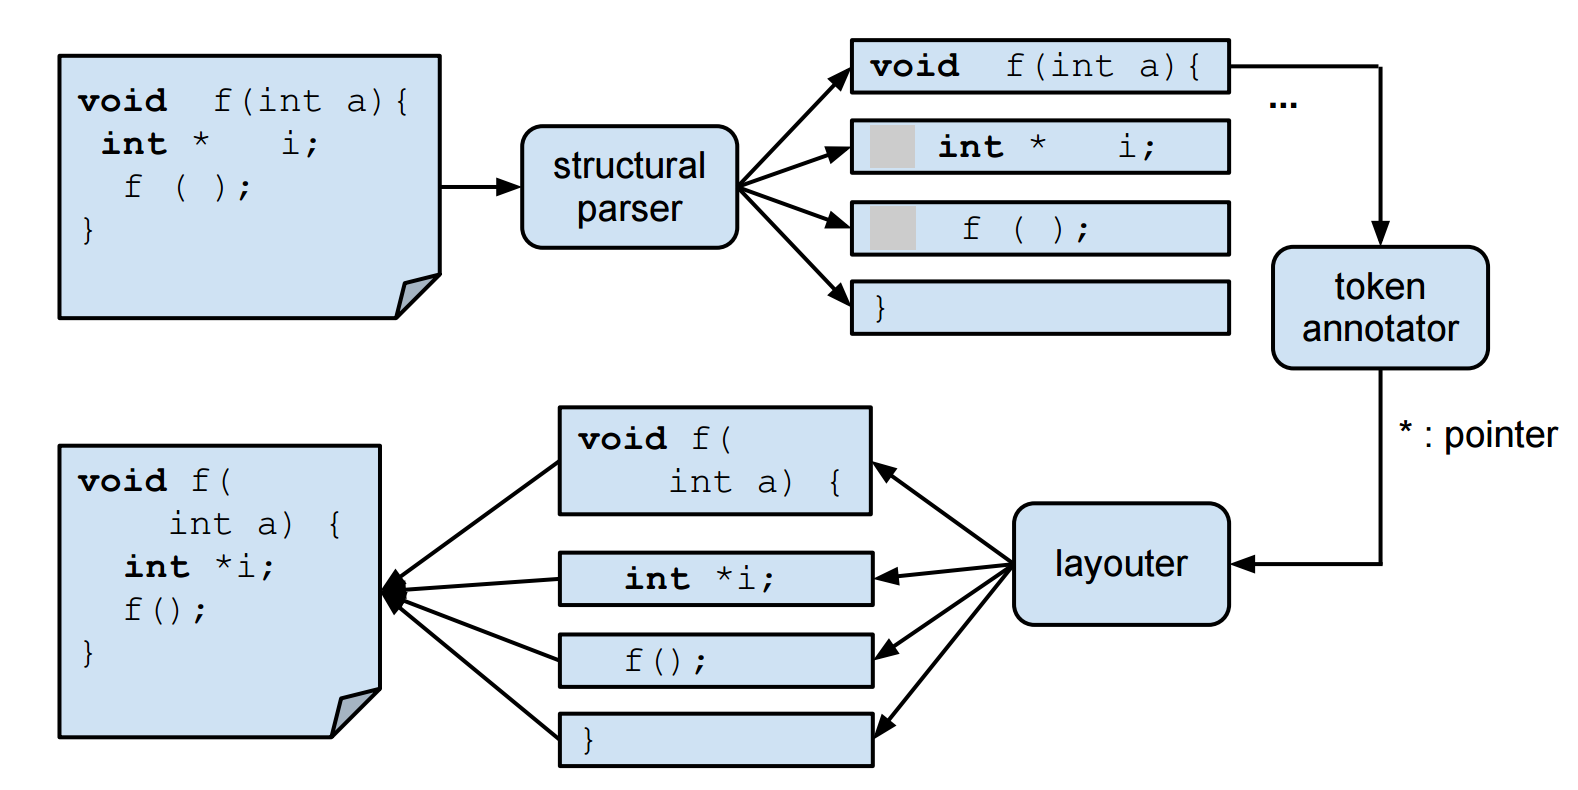
\includegraphics[width=0.9\textwidth]{img/clang-format.png}
  \caption{ClangFormat architecture}
  \label{fig:clang_format}
\end{figure}
The main components are the \emph{structural parser} and the \emph{layouter}.

ClangFormat employs a structural parser to split source code into a sequence of \emph{unwrapped-lines}.
An unwrapped line is a statement that should fit on a single line if given sufficient line length.
A key feature of unwrapped lines is that they should not influence other unwrapped lines.
The parser is lenient and parses even syntactically invalid code.
The parsed unwrapped lines are passed onto the layouter.

The ClangFormat layouter uses a novel approach to implement line wrapping.
Each line break is assigned a penalty according to several rules such as nesting and token type.
At each token, the layouter can choose to continue on the same line or break.
This forms an acyclic weighted directed graph with the first token of an unwrapped line being the root and all paths ending at the last token of the unwrapped line.
The layouter uses Dijkstra's\autocite{dijkstra_note_1959} shortest path algorithm to find the layout that has the lowest penalty.
To obtain good performance, the layouter uses several domain specific optimizations to minimize the search space.

Despite being seemingly language independent, ClangFormat does not leverage the language agnostic formatting techniques described section~\ref{sec:agnostic}.
Support for each language has been added as ad-hoc extensions to the ClangFormat parser and layouter.
ClangFormat supports a variety of configuration options, including 6 out-of-the-box styles based on coding styles from Google, LLVM and other well-known organizations.

A notable feature of ClangFormat is that it's opinionated.
ClangFormat produces well-formatted output for even the most egregiously formatted input.
Listing~\ref{lst:clang_opinion} shows an offensively formatted C++ code snippet.
\lstinputlisting[label={lst:clang_opinion}, float, caption=Unformatted C++ code]{code/terrible.cpp}
Listing~\ref{lst:clang_opinion2} shows the same snippet after being formatted with ClangFormat.
\lstinputlisting[label={lst:clang_opinion2}, float, caption=ClangFormat formatted C++ code]{code/target/unterrible.cpp}
ClangFormat is opinionated in the sense that it does not respect the user's line breaking decisions.
This feature makes it possible to ensure that all code follows the same style guide, regardless of author.

\subsubsection{dartfmt}
Dartfmt\autocite{nystrom_dart_style_2014} code formatter for the Dart programming language, developed at Google.
Like ClangFormat, dartfmt has a line length setting and is opinionated.
Bob Nystrom, the author of dartfmt, discusses the design of dartfmt in an excellent post\autocite{nystrom_hardest_2015} on his blog.
In his post, Nystrom argues that the design of a code formatters is significantly complicated by a column limit setting.
The line wrapping algorithm in dartfmt employs a \emph{best-first search}\autocite{pearl_heuristics:_1984},
a minor variant of the shortest path search in ClangFormat.
As with ClangFormat, a range of domain-specific optimizations were required to make the search scale for real-world code.
Listing~\ref{lst:dead_end} shows an example of such an optimization, \emph{avoiding dead ends}.
\lstinputlisting[label={lst:dead_end}, float, caption=Avoid dead ends]{code/dead-end.dart}
The snippets exceeds the 35 characters column limit.
A plain best-first search would explore a variety of different formatting layouts inside the argument list of \texttt{firstCall}.
However, the call to \texttt{firstCall} already fits on a line and there is no need to explore line breaks inside its argument list.
The dartfmt optimized search is able to eliminate such dead ends and quickly figure out to break before the \texttt{"long argument string"} literal.


\subsubsection{gofmt}
Gofmt\autocite{gofmt94:online} is a code formatter for the Go programming language, developed at Google.
Gofmt is noteworthy for its heavy adoption by the Go programming community.
Official Go documentation\autocite{CodeR59:online} claims that almost all written Go code is formatted with gofmt.
Moreover, besides formatting, gofmt is used to automatically migrate Go codebases from legacy versions to new source-incompatible releases.
However, gofmt supports neither a column limit nor an opinionated setting.
Line breaks are preserved in the user's input.
For example, listing~\ref{lst:gofmt} shows a Go program that was adapted from listing~\ref{lst:unformatted} in the introduction.
\lstinputlisting[label={lst:gofmt}, caption=Gofmt example input/output]{code/target/gofmt.go}
The output of running gofmt through listing~\ref{lst:gofmt} is identical to the input.
This un-opinionated behavior may be desirable for many software developers,
since it gives the programmer flexibility to choose a different layout for each argument list.
However, this thesis will not focus on such behavior.

% TODO?
% \subsubsection{rustfmt} 

\subsubsection{scalariform}
Scalariform\autocite{russell_scalariform_2010} is a widely used code formatter for Scala.
Scalariform does an excellent job of tidying common formatting errors and it supports a variety of configuration options.
Scalariform is also impressively fast, it can format large files with over 4.000 lines of code in under 250 milliseconds on a modern laptop.
However, like other code formatters such as gofmt, Scalariform lacks two key features: a line length and opinionated setting.

Firstly, the line length setting is necessary to implement many popular coding styles in the Scala community.
For example, the Spark\autocite{xin_spark_2015} and Scala.js\autocite{doeraene_scala.js_2015} coding styles have 100 character and 80 character column limits, respectively.
As we have learned from other code formatters, adding a line length setting is non-trivial and would require a significant redesign of Scalariform.

Secondly, the lack of an opinionated setting makes it impossible to enforce certain coding styles.
For example, the Scala.js coding style enforces \emph{bin-packing}, where arguments should be arranged compactly up to the column length limit.
Listings~\ref{lst:bin_pack} and~\ref{lst:non_bin_pack} shows an example of bin packing enabled and disabled, respectively.

\begin{minipage}{.45\textwidth}
  \lstinputlisting[label={lst:bin_pack}, caption=Bin-packing]{code/bin-pack.scala}
\end{minipage}
\hfil
\begin{minipage}{.45\textwidth}
  \lstinputlisting[label={lst:non_bin_pack}, caption=No bin-packing]{code/non-bin-pack.scala}
\end{minipage}

Since Scalariform preserves the line breaking decisions from the input,
Scalariform has no setting to convert formatted code like in listing~\ref{lst:non_bin_pack} to the code in listing~\ref{lst:bin_pack}.

\section{Algorithms}\label{sec:algorithms}
This chapter describes how scalafmt formats Scala code.
We will see that scalafmt's design is inspired by ClangFormat and dartfmt.
However, we believe our design makes a valuable contribution in that it leverages functional programming principles to maximise code reuse and extensibility.

\subsection{Design}
Figure~\ref{fig:architecture} shows a broad architectural overview of scalafmt.
\begin{figure}
  \centering
  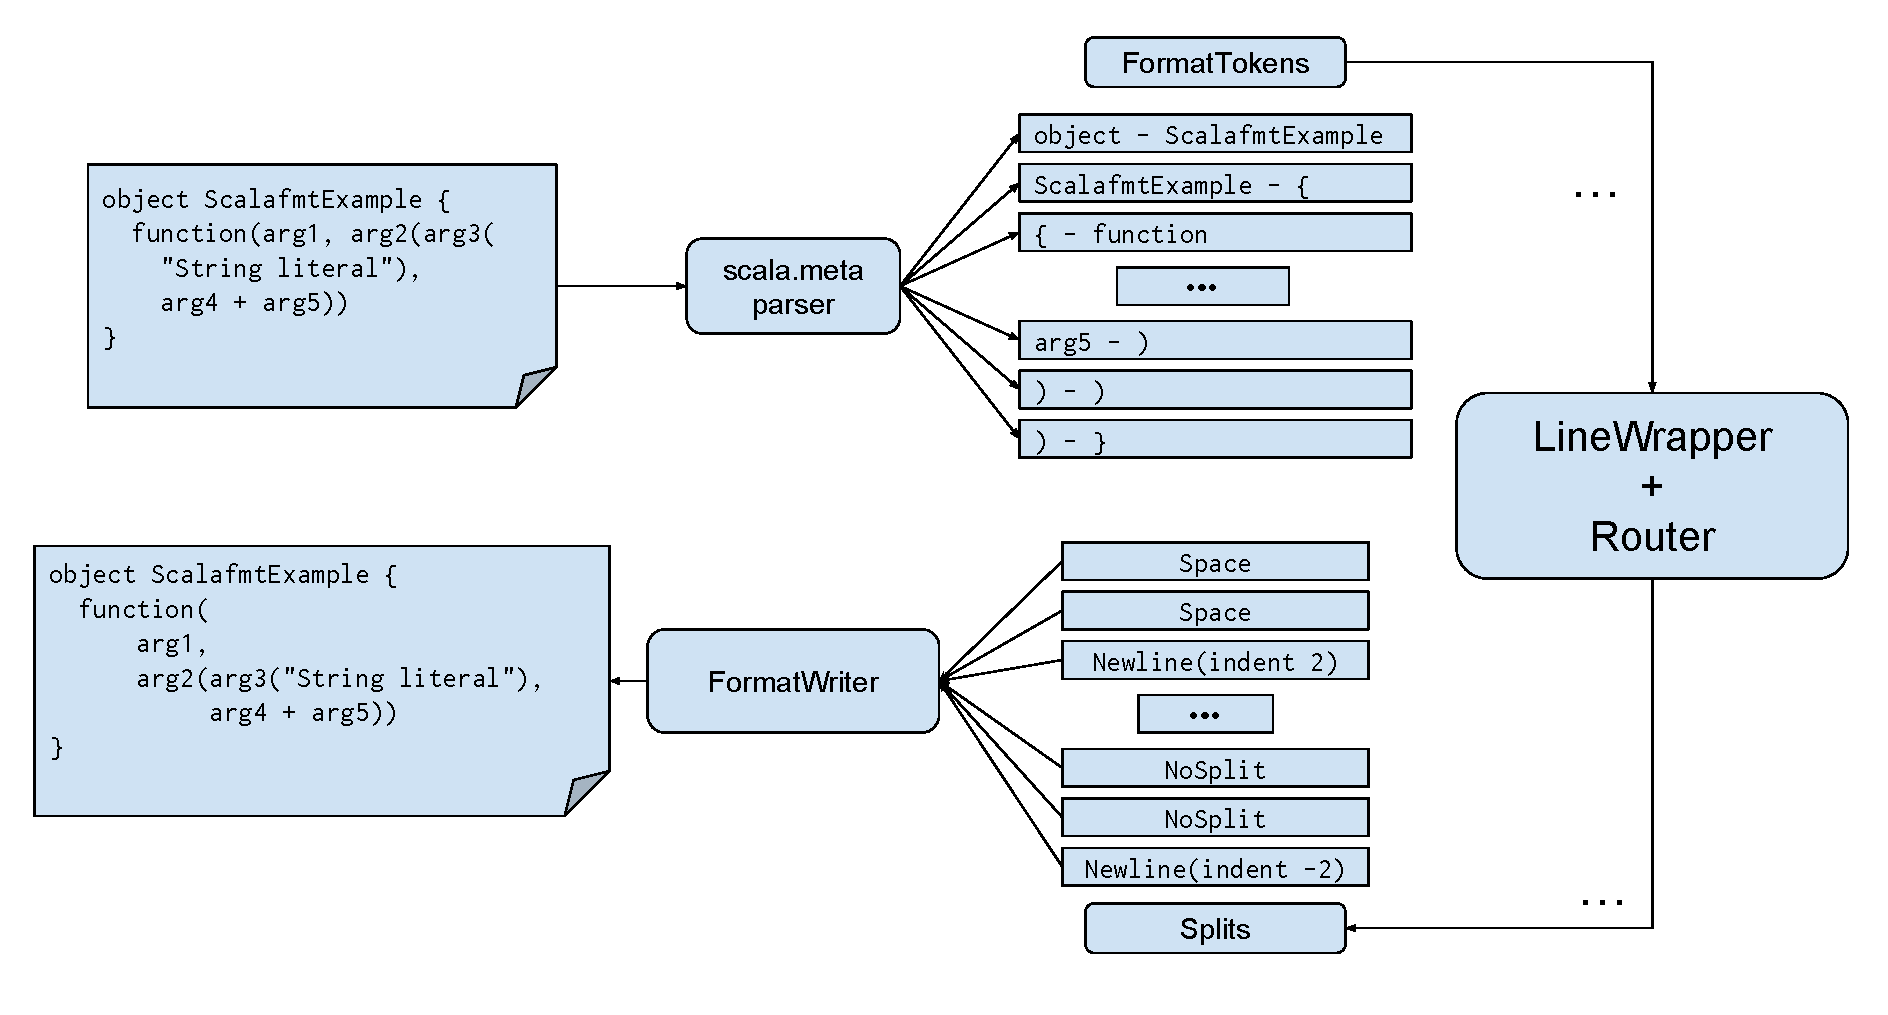
\includegraphics[width=\textwidth]{img/architechture.pdf}
  \caption{Scalafmt architecture}
  \label{fig:architecture}
\end{figure}
First, scalafmt parses a source file using scala.meta.
Next, we feed a sequence of \emph{FormatToken} data types into a \emph{LineWrapper}.
The LineWrapper uses a \emph{Router} to construct a weighted directed graph and run a best-first search to find an optimal formatting layout for the whole file.
Finally, the LineWrapper feeds a sequence of \emph{Split} data types into the \emph{FormatWriter}, which constructs a new reformatted source file.
The following sections explain these data types and abstractions in detail.

\subsection{Data structures}
Scalafmt leverages a few carefully designed data structure to allow an implementation that emphasizes correctness and maintainability.

\subsubsection{FormatToken}
A \emph{FormatToken} is a pair of two non-whitespace tokens.
Listing~\ref{lst:format_token} shows the definition of the FormatToken data type.
\lstinputlisting[label={lst:format_token}, caption=FormatToken definition]{code/format_token.scala}
As shown in the architecture overview in figure~\ref{fig:architecture}, each token except the beginning and end of file tokens appear twice in the sequence of FormatTokens: once as the \texttt{left} member and once as the \texttt{right} member.
In a nutshell, the job of the LineWrapper is to convert each FormatToken into a \emph{Split}

\subsubsection{Decision}\label{sec:decision}
A Decision is a pair of a FormatToken and a sequence of Splits.
Listing~\ref{lst:decision} shows the Definition of decision.
\lstinputlisting[label={lst:decision}, caption=Decision definition]{code/decision.scala}
The \emph{splits} member represents the possible splits that we can take at \emph{formatToken}.

\subsubsection{Policy}\label{sec:policy}
A \emph{Policy} is an enforced formatting layout over a region.
Listing~\ref{lst:policy} shows the definition of Policy.
\begin{minipage}{\linewidth}
  \lstinputlisting[label={lst:policy}, caption=Policy definition]{code/policy.scala}
\end{minipage}
A Policy is a partial function that should be applied to future Decisions up until the \emph{expire} token.
Policies easily compose using the Scala standard library \texttt{orElse} and \texttt{andThen} methods on PartialFunction\footnote{
  Careful eyes will observe that Policy is in fact a monoid with the empty partial function as identity and function composition as associative operator.}.
% The \texttt{isProhibitive} member annotates whether this policy can possibly eliminate Splits from future Decisions.
% This is necessary for an optimization explained in section~\ref{sec:dequeue}.
Policies enable a high-level way to express arbitrary formatting layouts over a region of code.

\subsubsection{Indent}\label{sec:indent}
An \emph{Indent} describes indentation over a region of code.
\lstinputlisting[label={lst:indent}, caption=Indent definition]{code/indent.scala}
Listing~\ref{lst:indent} shows the definition of Indent along with the algebraic data type \emph{Length}.
Length can either be \texttt{Num(n)} where $n$ represents an explicit number of spaces to indent by or \texttt{StateColumn} which is a placeholder the number of spaces required to vertically align by the current column.
Indent is type parameterized by Length so that, at some point, we can replace StateColumn placeholders with Nums to obtain a concrete number.
For example, given a scala.meta tree \texttt{expr}, the definition \texttt{Indent(Num(2), expr.tokens.last, inclusive=true)}
increases the indentation level by 2 spaces up to and including the last token of \texttt{expr}.
The \texttt{inclusive} member is set to false when the indentation should expire before the expire token, for example in a block wrapped by curly braces, since the closing curly brace should not be indented by 2 spaces.
The StateColumn placeholder is required to allow memoization of Splits, which is critical for performance reason as explained in section~\ref{sec:router} on the \emph{Router}.

\subsubsection{Split}
A \emph{Split} represents a (possibly empty) whitespace character to be inserted between two non-whitespace tokens.
Listing~\ref{lst:split} shows the rather intricate definition of the Split data type\footnote{
  For clarity reasons, a few less important members have been removed from the actual Split definition.}.
\begin{minipage}{\linewidth}
  \lstinputlisting[label={lst:split}, caption=Split definition]{code/split.scala}
\end{minipage}
The Split data type went through several generations of design before reaching its current structure.
Each member serves an important role.
The most important member of the Split type is the \emph{modification}.
A modification must be one of \texttt{NoSplit}, \texttt{Space} and \texttt{Newline}.
The \emph{cost} member represents the penalty for choosing this split.
The \emph{optimalToken} member enables an optimization explained in section~\ref{sec:optimal}.
The \emph{indents} member contains the indentation layers that this splits adds.
The \emph{line} member allows a powerful debugging technique explained in section~\ref{sec:router}.
The \emph{policy} and \emph{indents} members are explained in sections~\ref{sec:policy} and~\ref{sec:indent}, respectively.

\subsubsection{State}
A \emph{State} is a partial formatting solution during by the best-first search.
Listing~\ref{lst:state} shows the definition of the State class and companion object.
\begin{minipage}{\linewidth}
  \lstinputlisting[label={lst:state}, caption=State definition]{code/state.scala}
\end{minipage}
Observe the similarity of State and Split.
A State contains various summaries calculated from the \texttt{splits} member.
The summaries are necessary for performance reasons in the best-first search.
Observe that the indents are type parameterized by \texttt{Num}, meaning they only contain concrete indentations and no \texttt{StateColumn} indents.
The \texttt{indentation} member is the sum of all currently active indents and \texttt{column} represents how many characters have been consumed since the last newline.
The State class extends the \texttt{Ordered} trait to allow for efficient polling from a priority queue.
The \texttt{compare} method orders States firstly by their \texttt{totalCost} member, secondly by \texttt{splits.length} -- how many FormatTokens have been formatted -- and finally breaking ties by the \texttt{indentation}.
The method \texttt{nextState} calculates a penalty for characters that overflow the column limit and prepares
The method is implemented as efficiently as possible since the method is on a hot path in the best-first search.

, new summaries to instantiate a new State.
\subsection{LineWrapper}
The LineWrapper is responsible for turning FormatTokens into Splits.
To accomplish this, the LineWrapper employs a \emph{Router} and a best-first search.

\subsubsection{Router}\label{sec:router}
The Router's role is to produce a Decision given a FormatToken.
Figure~\ref{fig:router} shows all possible formatting layout for the small input \texttt{val x = y + z}.
\begin{figure}
  \centering
  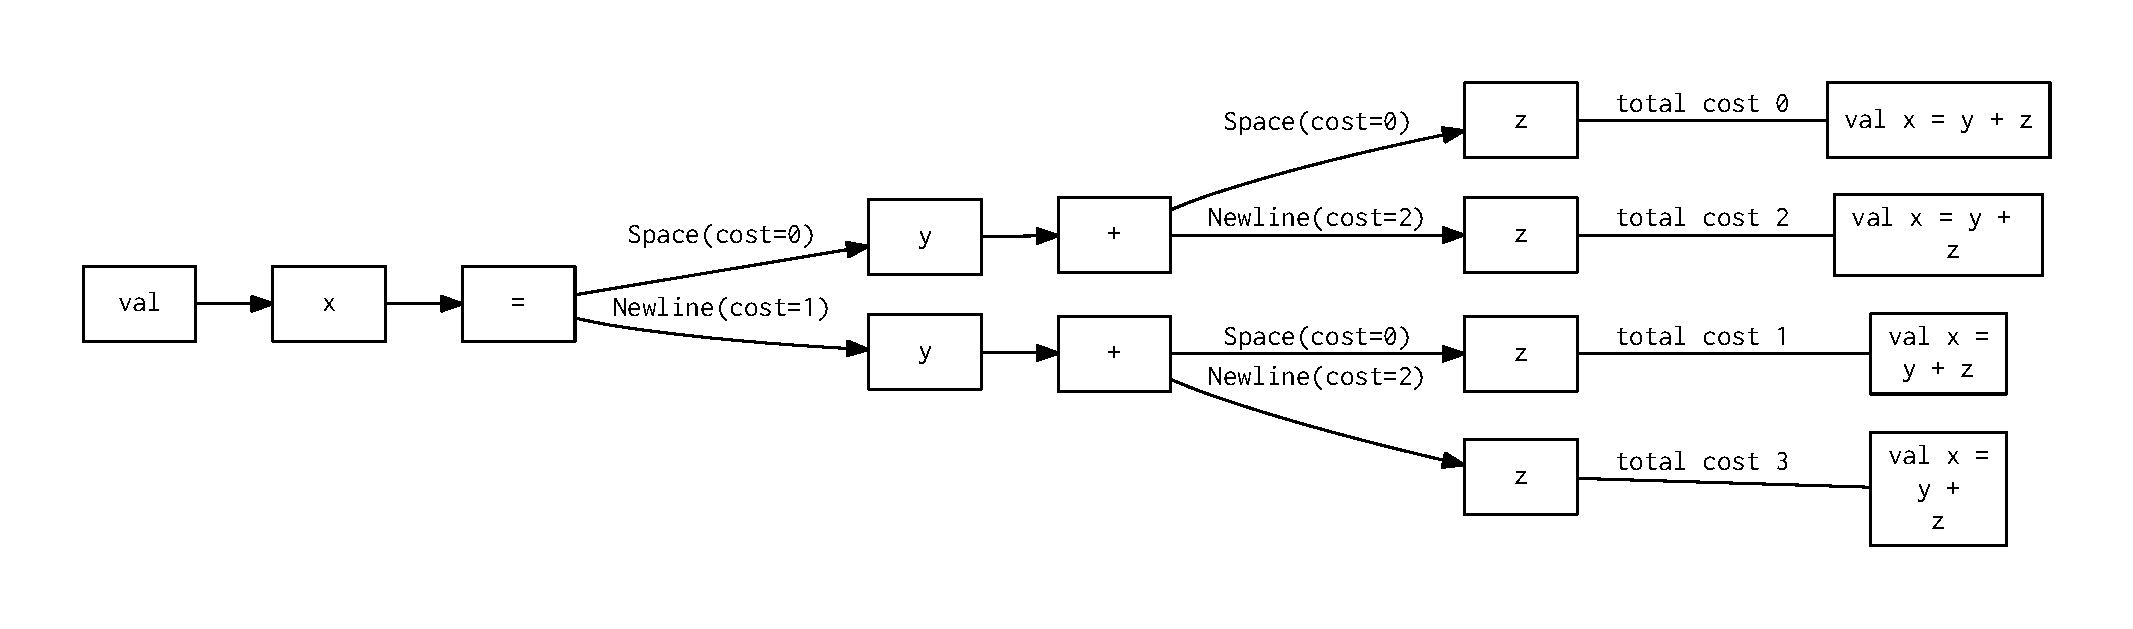
\includegraphics[width=\textwidth]{target/router.pdf}
  \caption{Example graph produced by Router}
  \label{fig:router}
\end{figure}
In this figure, the Router is the planner that chooses which nodes open up multiple branches (\texttt{=} and \texttt{+}) and which nodes have one exit edge only.
This is no easy task since a FormatToken can be any pair of two tokens.
How do we go about implementing a Router?

The Router is implemented as one large pattern match on a FormatToken.
Listing~\ref{lst:match} shows how to pattern match on a FormatToken.
\lstinputlisting[label={lst:match}, caption=Pattern matching on FormatToken]{code/match.scala}
The pattern \texttt{\_: `=`} matches a scala.meta token of type \texttt{`=`}.
The underscore \texttt{\_} ignores the underlying value.
Keyword is a super-class of all scala.meta keyword token types.
Now, a good observer will notice that this pattern match can quickly grow unwieldy long once you account for all of Scala's rich syntax.
How does this solution scale?
Also, once the match grows bigger how can we know from which case each Split origins?
It turns out that Scala's pattern matching and scala.meta's algebraically typed tokens are able to help us.

The Scala compiler can statically detect unreachable code.
If we add a case that is already covered higher up in the pattern match, the Scala compiler issues a warning.
For example, listing~\ref{lst:exhaustive} shows an example where the compiler issues a warning.
\lstinputlisting[label={lst:exhaustive}, caption=Unreachable code]{code/exhaustive.scala}
Here, we accidentally match on a FormatToken with an \texttt{else} keyword on the right which will never match because we have a broader match on a Keyword higher up.
In this small example, the bug may seem obvious but once the Router grows bigger the compiler becomes unmissable.
However, this still leaves us with the second question of finding the origin of each Split.
Scala macros\autocite{burmako2013scala} and implicits\autocite{oliveira2010type} come to the rescue.

The source file line number of where a Split is instantiated is automatically attached on each Split.
Remember in listing~\ref{lst:split} that the Split case class had an implicit member of type \texttt{sourcecode.Line}.
Sourcecode\autocite{lihao91:online} is a tiny Scala library to extract source code metadata from your programs.
The library leverages Scala macros and implicits to unobtrusively surface useful information such as line number of call sites.
Listing~\ref{lst:sourcecode} shows how this works.
\lstinputlisting[label={lst:sourcecode}, caption=Extracting line number from call site]{code/sourcecode.scala}
When a \texttt{sourcecode.Line} not passed explicitly as an argument to Split's constructor, the Scala compiler will trigger its implicit search to fill the missing argument.
The \texttt{sourcecode.Line} companion contains an implicit macro that generates a Line instance from an extracted line number.
Take a moment to appreciate how these two advanced features of the Scala programming language enable a very powerful debugging technique.
The scalafmt router implementation contains 88 cases and spans over 1.000 lines of code.
The ability to trace the origin of each Split has been indispensable in the development of the Router.
% Once the Router can produce Decisions, we can run a best-first search to choose the optimal splits.

\subsubsection{Best-first search}
The Decisions from the Router produce a directed weighted graph, as demonstrated in figure~\ref{fig:router}.
To find the optimal formatting layout, our challenge is to find the cheapest path from the root node to a final node.
The best-first\autocite{pearl_heuristics:_1984} algorithm is an excellent fit for the task.

Best-first search is a graph search algorithm to efficiently traverse a directed weighted graph.
The objective is reach the final token and once we reach there, we terminate the search because we're guaranteed no other solution is better.
Algorithm~\ref{alg:bfsv1} shows a first attempt\footnote{
  Unfortunately, we make heave use of mutation since graph search algorithms typically don't lend themselves well to functional programming principles.
} to adapt a best-first search algorithm to the data structures and terminologies introduced so far.
\begin{algorithm}
  \caption{Scalafmt best-first search, first approach}\label{alg:bfsv1}
  \lstinputlisting[nolol]{code/bfsv1.scala}
\end{algorithm}
In the best case, the search always chooses the cheapest splits and the algorithm runs in linear time.
Observe that the router is responsible for providing well-behaved splits so that we never hit on the error condition after the while loop.
Excellent, does that mean the search is complete?
Absolutely not, this implementation contains several serious performance issues.

Algorithm~\ref{alg:bfsv1} is exponential in the worst case.
For example, listing~\ref{lst:exponential} shows a tiny input that triggers the search to explore over 8 million states.
\lstinputlisting[label={lst:exponential}, caption=Exponential running time]{code/exponential.scala}
Even if we could visit 1 state per microsecond --- reality is closer to 10 states/microsecond ---  the search will take almost 1 second to complete.
This is unacceptable performance to format only 2 lines of code.
Of course, we could special-case long comments, but that would only provide us a temporary solution.
Instead, like with ClangFormat and dartfmt, we must apply several domain specific optimizations.
In the following section, we discuss the optimizations that have shown to work well for scalafmt.

\subsection{Optimizations}
This section explains the most important domain-specific optimizations that were required to get acceptable performance for scalafmt.
We will see that some optimizations are quite ad-hoc and require some creative workarounds.

\subsubsection{dequeueOnNewStatements}\label{sec:dequeue}
Once the search reaches the beginning of a new statement, empty the priority queue.
Observe that the formatting layout for each statement is independent from the formatting layout of the previous statement.
Consider listing~\ref{lst:dequeue}.
\lstinputlisting[label={lst:dequeue}, caption=Two independent statements]{code/dequeue.scala}
Both statements exceed the column limit, which means that the search must back-track to some extent.
However, once the search reaches \texttt{statement2} we have already found an optimal formatting layout for \texttt{statement1}.
When we start backtracking in \texttt{statement2}, there is no need to explore alternative formatting layouts for \texttt{statement1}.
Instead, we can safely empty the search queue once we reach the \texttt{statement2} token.

The \texttt{dequeueOnNewStatements} optimization is implemented by extending algorithm~\ref{alg:bfsv1} with an if statement.
Algorithm~\ref{alg:dequeue} shows a rough sketch of how this is done.
\begin{algorithm}
\caption{dequeueOnNewStatements optimization}\label{alg:dequeue}
  \lstinputlisting[nolol]{code/dequeue-alg.scala}
\end{algorithm}
With an empty queue, we ensure the search backtracks only as far back as is needed.
The \texttt{statementStarts} variable contains all tokens that begin a new statement.
To collect those tokens, we traverse the syntax tree of the input source file and select the first tokens of each statement of a block, each case in a partial function, enumerator in a for comprehension and so forth.
The actual implementation is quite elaborate and is left out of this thesis for clarity reasons.
Unfortunately, our optimization has one small problem.

Algorithm~\ref{alg:dequeue} may dequeue too eagerly inside nested scopes, leading the search to hit the error condition.
Listing~\ref{lst:noopt} shows an example where this happens.
\lstinputlisting[label={lst:noopt}, caption=Overeager dequeueOnNewStatements]{code/noopt.scala}
Remember that each case of a partial function starts a new statement.
The \texttt{dequeueOnNewStatements} optimization will dequeue the queue on the first state that reaches the \texttt{case} token.
In this example, the first state to reach the \texttt{case} token will have a strict Policy that disallows newlines up until the closing parenthesis.
However, we must insert a newline after the comment.
This causes the search to terminate too early and reach the error condition.
By inspecting where this problem occurred, we came up with a simple rule to identify regions where the \texttt{dequeueOnNewStatements} optimization should be disabled.
The simple rule is to never run \texttt{dequeueOnNewStatements} inside a pair of parentheses.
In section~\ref{sec:tooling}, we discuss techniques we used to be confident that this rule indeed works as intended.
In the following section (\ref{sec:recurseOnBlocks}) we explain the \texttt{recurseOnBlocks} optimization, which allows us to reenable \texttt{dequeueOnNewStatements} for selected regions inside parentheses.

\subsubsection{recurseOnBlocks}~\label{sec:recurseOnBlocks}
If the \texttt{dequeueOnNewStatements} optimization is disabled and we start a new block delimited by curly braces, recursively run the best-first search inside the block.
The intuition here is that by recursively running the best-first search, we keep the priority queue small at each layer of recursion.
This allows us to run aggressive optimizations such as \texttt{dequeueOnNewStatements}.

The \texttt{recurseOnBlocks} optimization enables scalafmt to handle idiomatic Scala code where large bodies of higher order functions and blocks are passed around as arguments.
Remember from section~\ref{sec:scala} that  Scala makes it syntactically convenient to in higher order functions as arguments to other functions.
Listing~\ref{lst:recurse} shows an example where this happens and we trigger the \texttt{recurseOnBlocks} optimization.
\lstinputlisting[label={lst:recurse}, caption=recurseOnBlocks example]{code/recurse.scala}
The \texttt{dequeueOnNewStatements} optimization is disabled inside argument list.
The priority queue grows out bounds because the higher order function can have an arbitrary number of statements.

To implement the \texttt{recurseOnBlocks} optimization, we add an extension to algorithm~\ref{alg:bfsv1}.
Algorithm~\ref{alg:recurse} shows a rough sketch of how \texttt{recurseOnBlocks} is implemented.
\begin{algorithm}
\caption{recurseOnBlocks optimization}\label{alg:recurse}
  \lstinputlisting[nolol]{code/recurse-alg.scala}
\end{algorithm}
We change the signature to accept a starting State and token where we stop the search.
Observe that we guard against infinite recursion by not making a recursive call on \texttt{start.formatToken}.
With \texttt{recurseOnBlocks} and \texttt{dequeueOnNewStatements}, we have solved most problems caused by independent statements affecting the formatting layouts of each other.
Next, we leverage recursion again to help the search queue stay small.

\subsubsection{OptimalToken}\label{sec:optimal}
An OptimalToken is a hint from a Split to the best-first search that enables the search to early eliminate competing Splits.
Recall from listing~\ref{lst:split} that a Split has an \texttt{optimalToken} member.
Listing~\ref{lst:optimalToken} shows the definition of OptimalToken.
\lstinputlisting[label={lst:optimalToken}, float, caption=OptimalToken definition]{code/optimalToken.scala}
When the best-first search encounters a Split with a defined OptimalToken,
the best-first search makes an attempt to reach that token with a budget of 0 cost.
If successful, the search can eliminate the competing Splits.
If unsuccessful and the \texttt{killOnFail} member is true, the best-first search eliminates the Split.
Otherwise, the best-first search continues as usual.

By eliminating competing branches, we drastically minimize the search space.
Listing~\ref{lst:optimal} shows an example where the OptimalToken can be applied.
\lstinputlisting[label={lst:optimal}, float, caption=OptimalToken example]{code/optimal.scala}
Scalafmt supports 4 different ways to format call-site function applications.
This means that there will be $4^N$ number of open branches when the search reaches \texttt{UserObject} $N$.
To overcome this issue, we define an OptimalToken at the closing parenthesis.
The best-first search successfully fits the argument list of each \texttt{UserObject} on a single line, and eliminates the 3 other competing branches.
This makes the search run in linear time as opposed to exponential.

To implement the \texttt{OptimalToken} optimization, we add an extension to algorithm~\ref{alg:recurse}.
Algorithm~\ref{alg:optimal} sketches how the extension works.
\begin{algorithm}
  \caption{OptimalToken optimization}\label{alg:optimal}
  \lstinputlisting[nolol]{code/optimalToken-alg.scala}
\end{algorithm}
The \texttt{bestFirstSearch} method has a new \texttt{maxCost} parameter, which is the highest cost that a new splits can have.
Next, if a Split has defined an \texttt{OptimalToken} we make an attempt to format up to that token.
If successful, we update \texttt{optimalFound} variable to eliminate other Splits from being added to the queue.
If unsuccessful and \texttt{killOnFail} is true, we eliminate the Split that defined the OptimalToken.
A straightforward extension to this algorithm would be to add a \texttt{maxCost} member to the \texttt{OptimalToken} definition from listing~\ref{lst:optimalToken}.
However, this has not been necessary for scalafmt.

\subsubsection{pruneSlowStates}
The pruneSlowStates is a optimization that eliminates states that progress slowly.
A state progresses slowly if it visits a token after other equally or less expensive states.
The insight is that if two equally expensive states visit the same token, the first state to visits that token typically produces a better formatting layout.

By eliminating slow states, we obtain a better formatting output in addition to minimizing the search space.
Listing~\ref{lst:slow} shows two equally expensive formatting solutions where one solution is fast and other is slow.
\lstinputlisting[label={lst:slow}, caption=Slow states]{code/slow.scala}
Of course, the line break after \texttt{g +} could be more expensive than the line break after \texttt{c +}.
Instead, the Router is free to assign an identical cost to both line breaks and let \texttt{pruneSlowStates} take care of eliminating the slow state.

The \texttt{pruneSlowStates} is implemented as a extension to algorithm~\ref{alg:optimal}.
Algorithm~\ref{alg:slow} shows a rough sketch of how the extension works.
\begin{algorithm}[H]
  \caption{pruneSlowStates optimization}\label{alg:slow}
  \lstinputlisting[nolol]{code/slow-alg.scala}
\end{algorithm}
Observe that this algorithm is transparent to the Router.
No special annotations are required from Splits.

\subsubsection{escapeInPathologicalCases}
Alas, despite our best efforts to keep the search space small, some inputs can still trigger exponential running times.
The \texttt{escapeInPathologicalCases} optimization is our last resort to handle such pathological inputs.
How do we detect that the search has encountered such a challenging input?

We detect the search space is growing out of bounds by tallying the number of visits per token.
If we visit the same token $N$ times, we can estimate the current branching factor to be around $log_2(N)$.
In scalafmt, we tune $N$ to be 256 so that the best-first search can split into two or more paths for up to 8 tokens.
When a token has been visited more than 256 times, we trigger the \texttt{escapeInPathologicalCases} optimization.
In the following paragraphs section, we present two alternative fallback strategies: \emph{leave unformatted} and \emph{best-effort}.

The simplest and most obvious fallback strategy is to leave the pathologically nested code unformatted.
This can be implemented by backtracing to the first token of the current statement and then reproduce the formatting input up to the last token of said statement.
This method is guaranteed to run linearly to the size of the input.
The responsibility is left to the software developer to a manually format her code, removing all the benefits of code formatting.
However, in some cases the software developer may prefer to get a decent yet suboptimal formatting output.

The best-effort fallback strategy applies heuristics to give a decent but suboptimal formatting output.
When a token is visited for the 256th time, we select two candidate states from the search queue and eliminate all other states.
The first state is the fastest state --- the state that has reached furthest into the token stream --- that is not bound a prohibitive single line policy.
Single line policies are policies that eliminate newline Splits.
The second state is the current state --- the slow state that visited the token for the 256th time.
The intuition is that the fast state has good formatting output so far but for is stuck on a challenging token for some reason.
The slow may paid a hefty penalty early causing it to move slowly but maybe the early penalty will yield a better output in the end.
Algorithm~\ref{alg:best-effort} shows an example of the best-effort strategy can be implemented as an extension to algorithm~\ref{alg:bfsv1}.
\begin{algorithm}
  \caption{best-effort fallback strategy}\label{alg:best-effort}
  \lstinputlisting[nolol]{code/best-effort.scala}
\end{algorithm}
The \texttt{isSafe} method on State returns true if the state contains prohibitive policies, derived from annotated metadata in Splits from the Router.
Observe that this algorithm will reapply the best-effort fallback until the search reaches the final token.
In scalafmt, we bound the number of this can happen with a final fallback to the unformatted strategy.

The unformatted and best-effort fallback strategies offer different trade-offs.
The unformatted strategy works well in a scenario where a software developer is available to manually fix formatting errors.
The best-effort strategy works well on computer generated code where just a modicum of formatting still greatly aid the legibility of the code.
Unfortunately, as we discuss in section~\ref{sec:testing}, we struggled to guarantee idempotency using the best-effort strategy.
This limitation renders the best-effort strategy useless in environments where code formatters are used to enforce a consistent coding style across a codebase.


\subsection{FormatWriter}
Recall from figure~\ref{fig:architecture}, the FormatWriter receives splits from the best-first search and produces a final output presented to the user.
In addition to reifying Splits, the FormatWriter runs three post-processing steps: \emph{docstring formatting}, \emph{vertical alignment} and \emph{stripMargin alignment}.

\subsubsection{Docstring formatting}\label{sec:docstring}
Docstrings are used by software developers to document a specific part of code.
Like in Java, docstrings in Scala start with the \texttt{/**} pragma and end with \texttt{*/}.
However, unlike in Java, the Scala community is split on whether new lines inside docstrings should align by the first or the second asterisk.
The official Scala Style Guide\autocite{Scala80:online} dictates that new lines should align by the second asterisk while the Java tradition is to align by the first asterisk.
The Scala.js\autocite{doeraene_scala.js_2015} and Spark\autocite{xin_spark_2015} style guides follow the Java conventions.
To accommodate all needs, scalafmt allows the user to choose either style.
To enforce that the asterisks are aligned according to the user's preferences,
the FormatWriter rewrites docstring tokens using simple regular expressions.

\subsubsection{stripMargin alignment}
The Scala standard library adds a \texttt{stripMargin} extension method on strings.
The method helps Scala developers write multiline interpolated and regular strings literals.
Listing~\ref{lst:stripMargin} shows an example usage of the \texttt{stripMargin} method.
\lstinputlisting[label={lst:stripMargin}, caption=stripMargin example]{code/stripMargin.scala}
After calling the method, the indentation and \texttt{|} character on line 3 are conveniently stripped away.
However, the hard-fought indentation can easily be lost when the string is moved up or down a scope during refactoring.
Scalafmt can automatically fix the issue.
In the FormatWriter, scalafmt rewrites string literals to automatically align the \texttt{|} characters with the opening triple quotes \texttt{"""}.
This setting is disabled by default since scalafmt has only syntactic information and cannot determine if the \texttt{stripMargin} invocation calls the standard library method or a user-defined method.

\subsubsection{Vertical alignment}


\section{Tooling}\label{sec:tooling}
\subsection{Heatmaps}
\subsection{Traceability}\label{sec:line}
\subsection{Configuration}
\subsubsection{maxColumn}
\subsubsection{binPacking}
\subsubsection{vertical alignment}
\subsection{Testing}~\label{sec:testing}
\subsection{Unit tests}
\subsection{Property based tests}
\subsubsection{AST Integrity}
\subsubsection{Idempotency}
\subsection{Regressions tests}

\section{Evaluation}\label{sec:evaluation}
Code formatting is inherently a subjective topic.
This introduces a challenge when evaluating a code formatter.
In this chapter, we will present measurements that we believe show the success of scalafmt.
We do not measure how well software developers perceive scalafmt formatted code.
Instead, we will focus on \emph{performance benchmarks} and \emph{user adoption}.

\subsection{Performance benchmarks}
This chapter measures scalafmt's raw formatting performance.
We first describe our test methodology and then present results from two different benchmarks: \emph{macro} and \emph{micro}.

\subsubsection{Setup}
The benchmarks are run on a Macbook Pro (Retina, 15-inch, Mid 2014) laptop with a quad-core 2.5 GHz Intel Core i7 processor, 256 KB L2 cache per core and 6 MB shared L3 cache.
The laptop has 16 GB 1600 MHz DDR3 memory.
The operating system is OS X El Capitan 10.11.5.
We run the benchmarks from the scalafmt commit id \href{https://github.com/olafurpg/scalafmt/tree/aff5e794dae4787b08243f8abb87a3ca4d907e40}{aff5e794} compiled against Scala 2.11.7, running on JVM version 8, update 91.
For accurate measurements, all benchmarks are run with the OpenJDK Java Microbenchmark Harness (JMH)\autocite{OpenJ38:online}.
JMH takes into account a variety of parameters that affect performance on the JVM.
The sbt-jmh\autocite{ktoso84:online} plugin makes it easy to integrate JMH with a Scala project.

To repeat the benchmarks, execute the \texttt{run-benchmarks.sh} script in the root directory of the scalafmt project.

\subsubsection{Macro benchmark}
The macro benchmark is designed to get insight on how scalafmt performs in a continuous integration setup.
For example, it is common to assert before code review that all source files are properly formatted.
For this benchmark we format the entire Scala.js codebase.
The codebase contains 915 source files and over 106 thousand lines of code, excluding blank lines and comments.
For accurate measurements, we run five iterations of the macro benchmark.
We compare the running time with Scalariform.

Table~\ref{tab:macro} shows the results from the macro benchmark.
\begin{table}
  \centering
  \caption{Results from macro benchmark.}\label{tab:macro}
  \begin{tabular}{lllll}
  Benchmark                &  Cores  &   Score  &   Error &  Units\\
  \hline
  \hline
  Parallel.scalafmt        &  4      &  14.616  &   0.632 &   s/op\\
  Parallel.scalariform     &  4      &   2.810  &   0.641 &   s/op\\
\hline
  Ratio &  & 5.20 &  & \\
  \\
  Synchronous.scalafmt     &  1      &  35.654  &   0.459 &   s/op\\
  Synchronous.scalariform  &  1      &   5.951  &   0.135 &   s/op\\
\hline
  Ratio &  & 5.99 &  & 
\end{tabular}

\end{table}
Scalafmt is almost 6x slower than Scalariform.
Why is the performance gap so big?
Is this gap acceptable for continuous integration setups?

We believe two factors contribute to the fact that scalafmt is 6x slower than Scalariform.
Firstly, preliminary results from profiling scalafmt reveal that micro-optimizing scalafmt could yield great performance improvements.
For example, over 30\% of the formatting time is dedicated to a pre-processing step --- unrelated to the best-first search --- that could be accomplished with minimal overhead during parsing inside scala.meta.
Other experiments indicate that scalafmt may speed up yet another 30\% by upgrading to the latest release of scala.meta\footnote{
  Scala.meta recently went through several non-source-compatible upgrades.
  This has made it difficult for scalafmt to keep up with the latest release.
}.
Secondly, scalafmt's formatting algorithm is more complex.
Scalafmt may try thousands of different formatting layouts to find an optimal formatting output.
In contrast, Scalariform's formatting algorithm is linear.

We believe the current performance is usable in a continuous integration setup, but would benefit greatly from performance improvements.
The current performance is usable because a typical diff in a code review touches only a few source files, and definitely far from the 106 thousand lines of code that we format in this macro benchmark.
On a smaller diffs, the gap between Scalariform and scalafmt is less pronounced.
However, it is worth considering that continuous integration setups may not have access to the same powerful hardware as we do in this benchmarks.
We estimate that scalafmt requires at least a 2-3x performance improvement to be integrated in continuous integration setups with less powerful hardware and projects that contains large amounts of code.


\subsubsection{Micro benchmark}
The micro benchmark is designed to get insight on how scalafmt performs in an interactive software developer workflow.
For example, many Scala developers configure SBT to reformat source files on every compilation.
Before we run the benchmark, we must find out how many lines of code a typical source file contains.

We performed a small study to learn the size of a typical source file.
We collected a sample of 3.2 million lines of code from 33 open source Scala projects.
Table~\ref{tab:macro_sample} shows the distribution of file sizes in our sample.
\begin{table}
  \centering
  \caption{Percentiles of lines of code per file in micro benchmark.}~\label{tab:macro_sample}
  \begin{tabular}{llllllll}
  25th & Median & Mean & 75th & 90th & 95th & 99th & Max\\
  \hline
  \hline
  16 & 46 & 106 & 113 & 248 & 400 & 945 & 11.723\\
  
\end{tabular}

\end{table}
Observe that over 90 percent of all files are rather small, or under 250 lines of code.
Only one percent of files contain more than 1.000 lines of code.
Still, we assume developers spend quite a lot of time editing such large files.

Using the results from our small study, we choose to run the micro benchmark on four files of varying sizes: small ($\sim$ 50 LOC), medium ($\sim$300 LOC), large ($\sim$1.000 LOC) and extra large ($\sim$4.500 LOC).
To minimize error margins, we run 10 warmup iterations followed by 10 measured iterations.
As in the macro benchmark, we compare the running time with Scalariform.
The micro benchmark is single threaded.

Table~\ref{tab:micro} shows the results from the micro benchmark.
\begin{table}
  \centering
  \caption{Results from micro benchmark.}\label{tab:micro}
  \input{target/micro.tex}
\end{table}
No surprise, scalafmt is again slower than Scalariform.
Is this performance gap acceptable for interactive software development?

We believe this performance is usable for occasional code formatting, but not suitable for a workflow that formats on every compilation.
Amazon famously showed that sales decreased by 1 percent for every 100ms increase in page load time\autocite{kohavi2007online}.
We believe similar principles apply to scalafmt, every additional millisecond decreases the utility of scalafmt.
Still, we believe with scalafmt's formatting output is appealing enough to outweigh the slow performance.
As we'll discuss in the following section, our users seem to agree.

\subsection{Adoption}\label{sec:adoption}
Scalafmt has received quite some attention since its release in early March, three months ago.
In this section we present the statistics we believe demonstrate that scalafmt is --- despite its young age --- already proving itself useful for the Scala community.
All data points are as of June 9th, 2016.

\subsubsection{Installations}
Scalafmt has been installed over 6.500 times.
  Table~\ref{tab:installs} shows the installation numbers for each official distribution channel.
  \begin{figure}
    \CenterFloatBoxes
    \begin{floatrow}
      \ffigbox
      {
\includegraphics[width=0.4\textwidth,angle=-90]{target/month.eps}}
      {\caption{Scalafmt installations by month by channel}\label{fig:installs}}
      \killfloatstyle
      \ttabbox{\begin{tabular}{lll}
  Channel          & Version  &  Installations\\
  \hline
  \hline
  IntelliJ         & v0.2.5   &  847            \\
                   & All      &  3.273\\
  Maven            & v0.2.5   &  788            \\
                   & All      &  2.657          \\
  Github           & v0.2.5   &  102            \\
                   & All      &  929            \\
\hline
  Sum        & v0.2.5   &  1.737          \\
                   & All      &  6.859          
\end{tabular}
 }{
        \caption{Download numbers for scalafmt.}\label{tab:installs}}
    \end{floatrow}
  \end{figure}
IntelliJ is the Jetbrains plugin repository\footnote{
  See \url{https://plugins.jetbrains.com/plugin/8236?pr=}
}.
The numbers represent absolute download numbers, not unique users.
Data is not available for how many users built scalafmt from source, so it is fair to estimate that the actual number of installation is even higher.
Observe that v0.2.5 was released 22 days ago, meaning it has been installed 80 times on average per day since its release.
Extrapolating from the v0.2.5 installations numbers, we expect that scalafmt currently has roughly 1.000 active users.

Figure~\ref{fig:installs} shows the growth in installations by month.
Observe that growth has doubled with each new month.
Github represented proportionally many installs in the first month but only represents a small fraction of installation in May.
Maven installations quadrupled in May, taking the lead from the IntelliJ plugin in April.
We believe this increase in Maven installations is caused by projects installing the scalafmt SBT plugin for every test run in a continuous integration setup.


\subsubsection{Other}
We present interesting data points from a variety of disparate data sources:
\begin{table}
  \hyphenpenalty=1000
  \caption{Open source libraries that have reformatted their codebase with scalafmt and their customized settings.}\label{tab:oss}
  \begin{tabular}{lp{90mm}}
    Project & Customized coding style \\
    \hline \hline
    Scala Native\tablefootnote{
      \url{https://github.com/scala-native/scala-native}} & \texttt{defaultWithAlign} base style,
                                                            80 character column limit,
                                                            Java docstrings. \\
    Scala.js dom\tablefootnote{
      \url{https://github.com/scala-js/scala-js-dom}}     & \texttt{Scala.js} base style:
                                                            80 character column limit,
                                                            vertical alignment on case arrows,
                                                            bin packed arguments/parameters/parent constructors,
                                                            Java docstrings. \\
    Fetch\tablefootnote{
      \url{https://github.com/47deg/fetch}}               & \texttt{defaultWithAlign} base style,
                                                            100 character column limit,
                                                            Scala docstrings. \\
    psp-std\tablefootnote{
      \url{https://github.com/paulp/psp-std}}             & Customized vertical alignment,
                                                            160 character column limit,
                                                            2 space continuation indent,
                                                            spaces in import curly braces,
                                                            Scala docstrings.

  \end{tabular}
\end{table}
\begin{itemize}
  \item Several popular open-source libraries have reformatted their codebases with scalafmt.
    Table~\ref{tab:oss} shows an incomplete list libraries that have so far taken the jump.
    Observe that all libraries take advantage of vertical alignment.
    Moreover, each library customize on top of the base \texttt{default} style.
    It is worth mentioning that all libraries except Scala.js dom are relatively new.
    We believe more mature libraries are slower to adopt such new technology.
  \item The scalafmt code repository has received contributions from 8 external contributors.
    Several of these contributions added non-trivial features to scalafmt, including
    new configuration flags and extensions to the Router.
  \item 34 unique users, excluding the author, have opened a total of 138 tickets on the scalafmt issue tracker.
  \item The scalafmt Gitter\footnote{See \url{https://gitter.im/olafurpg/scalafmt}} instant messaging channel has 47 members. The channel is used to informally discuss bugs, new features and more.
  \item The user documentation website\footnote{See \url{http://scalafmt.org}} has been visited 5.422 times with an average visit duration of 98 seconds.
\end{itemize}




\section{Discussion}
\subsection{Future work}
\subsection{Conclusion}

% \section{Related work}
% \subsection{Combinator based}
% \begin{enumerate}
%   \item Houghes 1995
%   \item Wadler 1999
% \end{enumerate}
% \subsection{Optimization-oriented}
% \begin{enumerate}
%   \item clang-format Dijkstra's 2010
%   \item dartfmt Best-first search 2014
%   \item rfmt 2015
% \end{enumerate}
% \begin{enumerate}
%   \item Optimal line breaking
%   \item Oppen
% \end{enumerate}

\pagebreak
\printbibliography{}

\end{document}


